\chapter{Bayesian Optimization}
Whereas traditional regression workflow is the following: From data, fit model parameters, make predictions using the parameters. 
The Bayesian framework allows us to skip the dependency of a single set of parameters and instead use all sets of parameters 
by treating the set of parameters as a random quantity, $\theta$. What is of interest is the predictive posterior distribution,  
\begin{align}\label{Predictive2}
    p(y|x, \mathcal{D})
\end{align}
% Before bringing the parameters/unknown quantities into play, we can ask: What quantities can we play
% with? This question is answered in two different ways in Gaussian process regression and Bayesian
% Neural network regression.

Bayesian optimization is essentially two steps: First, a probabilistic surrogate-model is fitted
to the available data $\mathcal{D}$ giving the predictive distribution \eqref{Predictive2}. Second,
the next sample point is chosen according to a so-called acquisition function, which in a sense
balance out the well-known concept, exploitation and exploration. Where exploitation will be chooing
the next point according to its expected improvement and exploration will be choosing the next point
in a region of high uncertainty and thereby help lower the overall uncertainty. We will first look at
the acquisition function used in this thesis, which is also the most commonly used: E   xpected improvement. 

\section{Acquisition function}

\subsection{Expected improvement}
A popular choice of acquisition function is expected improvement, 
$$EI(x) = \mathbb{E}_{p(y|x,\mathcal{D})}[\max(0, y_{\min}-y)]$$
this will only look at the expectation of the values $y$, which improves the current best value.

\begin{figure}[H]
    \centering
    \includegraphics[width=0.8\textwidth]{Pictures/expected_improvement_illustration.pdf}
\end{figure}

In the following deveration
we assume the predictive distribution can be approxiamted by a normal distribution dependent on
the point of interest $x$ and the data $\mathcal{D}$ (note for the GP
it is in fact not an approximation), 
$$p(y|x,\mathcal{D}) \approx \mathcal{N}(y|\mu(x,\mathcal{D}), \sigma^2(x,\mathcal{D}))$$ where we
will change to a less clumpsy notation $\mathcal{N}(y|\mu_x,
\sigma^2_x):=\mathcal{N}(y|\mu(x,\mathcal{D}), \sigma^2(x,\mathcal{D}))$. This is completely fine
since we $x$ is fixed (and $\mathcal{D}$ is fixed) when evaluating the expected improvement in a point
$x$. %  $\sigma_x := \sigma^2(x,\mathcal{D})$ and $\mu_x := \mu(x,\mathcal{D})$
%as evaluated functions, i.e. numbers. 
Furthermore, the density of
a standard normal distribution is denoted $\phi(\cdot):=\mathcal{N}(\cdot | 0,1)$, and the cumlative
density function (CDF) of a standard normal distribution is denoted, $\Phi(\cdot) :=
\int_{-\infty}^{\cdot} \phi(\epsilon)d\epsilon$. We will now see that the normal approximation
of the predictive distribution yiels closed form solution to the expected improvement function, 

\begin{align*}
    E_{p(y|x,\mathcal{D})}[\max(0,y_{\min}-y)] &= \int \max(0,y_{\min}-y) p(y|x,\mathcal{D}) dy\\
    &\approx \int \max(0,y_{\min}-y) \mathcal{N}(y|\mu_x, \sigma_x^2) dy\\
    &= \int_{-\infty}^{y_{\min}} (y_{\min}-y) \frac{1}{\sigma_x}\phi\left(\frac{y-\mu_x}{\sigma_x}\right) dy\\
    &= \int_{-\infty}^{\frac{y_{\min}-\mu_x}{\sigma_x}} (y_{\min}-\mu_x-\sigma_x\epsilon) \frac{1}{\sigma_x}\phi\left(\epsilon\right) \sigma_x d\epsilon\\
    &= \int_{-\infty}^u \sigma_x \cdot (u-\epsilon) \phi(\epsilon) d\epsilon\\
    &=  \sigma_x \cdot \left( u\cdot \int_{-\infty}^u \phi(\epsilon) d\epsilon +\int_{-\infty}^u (-\epsilon)  \phi(\epsilon) d\epsilon \right) \\
    &= \sigma_x [u\Phi(u)+ \phi(u)]
\end{align*}

where $u:=\frac{y_{\min}-\mu_x}{\sigma_x}$. To understand the identity $\phi(u) = \int_{-\infty}^u
(-\epsilon)  \phi(\epsilon) d\epsilon$ used in the last equality, we first see that the antiderivative
is $\phi(\epsilon) = \frac{1}{\sqrt{2\pi}} \exp(\frac{-\epsilon^2}{2})$,
\begin{align*}
    \frac{d}{d \epsilon} \phi(\epsilon) &=  \frac{1}{\sqrt{2\pi}}\frac{d}{d \epsilon} \exp(\frac{-\epsilon^2}{2})\\
    &=  \frac{1}{\sqrt{2\pi}}\exp(\frac{-\epsilon^2}{2})(-\epsilon)\\
    &= -\epsilon \phi(\epsilon)
\end{align*}
and evaluating the rieman integral is equivalent to evaluate the antiderivative in its boundaries, giving the 
solution, 
$$\int_{-\infty}^u
(-\epsilon)  \phi(\epsilon) d\epsilon = \left[\phi(\epsilon)\right]_{-\infty}^u = \phi(u)-0 = \phi(u)$$ 

We can also explicily write the expected improvement as, 
$$EI(x) = (y_{\min}-\mu_x)\Phi\left(\frac{y_{\min}-\mu_x}{\sigma_x}\right)+ \sigma_x
\phi\left(\frac{y_{\min}-\mu_x}{\sigma_x}\right)]$$
where the first part can be interpretted as exploitation (favouring points with a large improvement $I(x) := (y_{\min}-\mu_x)$)
and the second part can be seen a exploitation (favouring points with high uncertainty.)
taking the derivative with respect to $I(x) := (y_{\min}-\mu_x)$ and $\sigma_x$, we see that expected improvement is 
is increasing if the improvement grows or if the variance $\sigma_x$ grows, i.e
$$\frac{\partial EI(x)}{\partial I(x)} = \Phi\left(\frac{y_{\min}-\mu_x}{\sigma_x}\right) > 0, \hspace*{0.5cm} 
\frac{\partial EI(x)}{\partial \sigma_x} = \phi\left(\frac{y_{\min}-\mu_x}{\sigma_x}\right) >0$$ 
<obs mistake in the book!!!?>





\begin{align*}
    \mathbb{E}_{y_*|\textbf{x}_*,D_n}[\max(0,y_{\min}-y_*)] &= ??\\
    \mathbb{E}[\min(0,y_{\min}-y_*)|\textbf{x}_*,D_n] &= \int_{-\infty}^\infty \min(0,y_{\min}-y_*) p(y_*|\textbf{x}_*,D_n) dy_*\\
    &= \int_{-\infty}^{y_{\min}} (y_{\min}-y_*) p(y_*|\textbf{x}_*,D_n) dy_*\\
    &\approx \frac{1}{N} \sum_{\theta \in \Omega } [y_{\min}-f_\theta(x)]
\end{align*}

where $\Omega = \{\theta|f_{\theta}(x)< y_{\min}\}$

%\section{uncertainties}
%Alatoric vs epistemic uncertainties 

\subsection{Entropy search}
We then discuss the knowledge
gradient (Section 4.2), entropy search and predictive entropy search (Section 4.3) acquisition functions.
These alternate acquisition functions are most useful in exotic problems where an assumption made by
expected improvement, that the primary benefit of sampling occurs through an improvement at the point
sampled, is no longer true.


The entropy search (ES) (Hennig and Schuler, 2012) acquisition function values the information we have
about the location of the global maximum according to its differential entropy

ES seeks the point to evaluate that causes the largest decrease in differential entropy

(Recall from, e.g., Cover and Thomas (2012),
that the differential entropy of a continuous probability distribution p(x) is R
p(x) log(p(x)) dx, and that
smaller differential entropy indicates less uncertainty.)

Predictive entropy search (PES) (Hern´andezLobato et al., 2014) seeks the same point, but uses a reformulation of the entropy reduction objective
based on mutual information. Exact calculations of PES and ES would give equivalent acquisition functions, but exact calculation is not typically possible, and so the difference in computational techniques
used to approximate the PES and ES acquisition functions creates practical differences in the sampling
decisions that result from the two approaches. We first discuss ES and then PES.

Let x  be the global optimum of f. The posterior distribution on f at time n induces a probability
distribution for x
. Indeed, if the domain A were finite, then we could represent f over its domain by a
vector (f(x) : x ∈ A), and x
would correspond to the largest element in this vector. The distribution of
this vector under the time-n posterior distribution would be multivariate normal, and this multivariate
normal distribution would imply the distribution of x

. When A is continuous, the same ideas apply,
where x

is a random variable whose distribution is implied by the Gaussian process posterior on f



\section{surrogate model}
As mentioned in the previous sections, the first of two repeated steps in Bayesian optimization
is to create a good Bayesian regression model. %why not non bayesian regression? 
i.e. finding the probility of prediction for a arbitrary point $x$ given datapoints 
$\mathcal{D} = \{x_1, y_1, \dots, x_n, y_n\}$, 
 $$p(y|x,\mathcal{D})$$

The surrogate model of choise in Bayesian optimization is a Gaussian Process, and Bayesian Neural Network.
These are discriminative models, however, another approach, which we focus on in this project, is
to model $y$ and $x$ jointly in a so-called generative model.



\subsection{Discriminative model as surrogate model}
When talking about a probabilistic surrogate model we are always implicit talking about a
discriminative model: A model of the conditional distribution of the observation, $y$, 
conditional on $x$, i.e., 
$$p(y|x)$$
we also refer to this as the predictive distribution. Gaussian processes and Bayesian neural networks
are both discriminative models. There is no distribution over the input $x$, it is just given. 
This is indeed sufficient for a surrogate model, where we are interested in the predictive distribution. 

\subsection{Using a generative model as surrogate model}

Given a generative model over $x$ and $y$ paramitised with $\theta$, we are dealing with the joint distribution
$$p(x,y|\theta)$$
and we are interested in the condtional distribution of y given x, 
$$p(y|x, \theta_{y|x})$$
where we have put subscript on $\theta$ in order to jump up a level of abstraction since, 
in fact there is just a mapping between them $\theta_{y|x} := g(\theta, y, x)$ 

% $$\alpha p(y|x) + (1-\alpha) \mathcal{N}(0,1)$$

% so what should $\alpha$ be? Here we can find inspiration from a Poission point process. 


\begin{align*}
    p(y|x, \mathcal{D}) &= \int p(y|x,\theta_{y|x})p(\theta_{y|x}|\mathcal{D}) d\theta_{y|x}  \\
    &=  p(y|x,\hat \theta_{y|x})
\end{align*}
Where the last equation holds as we assume that $p(\theta_{y|x}|\mathcal{D})$ is a delta function
i.e. a point estimate with value $\hat \theta_{y|x}$. In the case of our Gaussian mixture model, 
we obtain a point estiamte from the EM algorithm for the variance $\Sigma_{y|k}$, mean value $\mu_{y|k}$ and proportion $\pi_{y|k}$
for each component $k = 1,2, \dots, K$
$$\hat \theta_{y|x} = (\hat\Sigma_{y|k}, \hat\mu_{y|k}, \hat\pi_{y|k})_{k=1}^K$$

However, we are not satisfied with the variance estimate for the regression, as it is way too small for areas with
no observed data. It is therefore necessary to manipulate the variance estimate accoring to that observation. 
We multiply the variance obtained using expectation-maximization on the joint distribution with the 
inverse of the probability of the data $x$, and control that the scaling factor is not going wild!

$$\hat\Sigma_{y|k} =\Sigma_{y|k}^{GMM} \frac{1}{\max(p(x), 0.01)}$$

In a way, this is manipulation in a Bayesian spirit, as we let prior and subjective knowledge influence the
variance prediction. 
\subsection{Inclusion of prior distribution}
The new conditional distribution is essentially a mixture between the old conditional and the prior distribution, 
$$\hat p(y|x) = \alpha_x p(y|x) + (1-\alpha_x)p_{prior}(y)$$
where we choose $\alpha_x := \frac{S(x)}{S(x)+1}$. A convex combination of distributions is a distribution, 
since 
\begin{align*}
    \int_y \hat p(y|x) dy &= \int_y \left[ \alpha_x p(y|x) + (1-\alpha_x)p_{prior}(y) \right] dy\\
     &= \alpha_x \int_y p(y|x)dy +(1-\alpha_x) \int_y p_{prior}(y)dy \\
     &= \alpha_x + (1-\alpha_x) = 1
\end{align*}
    
\subsection{Inclusion of prior distribution}
Since the prior predictive distribution and the predictive distribution both are assumed to be normal distributions, 
it is possible to simply let the parameters of the manipulated predictive distributions be a convex combination of the 
parameters. This will make the manipulation be more natural, and hopefully less coruptive. 
\begin{align*}
    \hat p (y|x) &=\mathcal{N}(y| \hat \mu, \hat\sigma^2)\\
    \hat \mu &= \alpha \cdot \mu_{y|x} + (1-\alpha) \cdot \mu_{prior}\\
    \hat \sigma^2 &= \alpha \cdot \sigma_{y|x}^2 + (1-\alpha) \cdot\sigma_{prior}^2
\end{align*}


\subsection{Inclusion of prior distribution}
The conditional distribution $p(y|x)$ obtained from using a Gaussian mixture model is without a prior, and
the predictive distribution yields a way too small uncertainty estimate in regions where there are no observations.
This is because the range of the Gaussian distribution continues throughout the entire space and even though the
joint distribution is very small in the region, the conditional distribution is normalized using the (very small) $p(x)$.
We, therefore, want to introduce a prior, which can rule over the conditional in regions where the probability is too
small. The first approach is simply to define a new conditional distribution, 
\begin{align}\label{manipulated_pred_dist}
    \hat p(y|x) &\propto S(x) \cdot p(y|x) + p_{prior}(y)
\end{align}
where the scaling function can be interpreted as the probability of the input $x$ is in the region
ball $x \in B_{\frac{1}{2}\Delta}(x)$, and the probability density is not just $p(x)$ but the
probability of the average mixture component, which is $K\cdot p(x)$, assuming the mixture is
dominated be a single component at the position $x$. We define the scaling as 
$$S(x):= K\cdot p(x)\cdot \Delta$$
% $p_K(x)$ is the marginal density of an average mixture component, i.e. 
% $$p(x) = \sum_{k=1}^K \gamma_k p_k(x) \implies p_K(x) = K \cdot p(x)$$
Next we need to normalize the manipulated predictive distribution in order to
make it a proper probability density, i.e., making sure it integrates to 1, 
$$\int S(x) \cdot p(y|x) + p_{prior}(y) dy =S(x)+1$$
so the we can easily update \eqref{manipulated_pred_dist} with an equality
sign by defining the manipulated predive distribution as, 
$$\hat p(y|x) = \frac{S(x) \cdot p(y|x) + p_{prior}(y)}{S(x)+1}.$$

In figure \ref{pred_dist_manipulation} the manipulated predictive 
distribution is illustrated under the influenced of different scalings. 
Note that if $S(x) = 0$ the manipulated distribution becomes the prior,
while in the limit $S(x) \rightarrow \infty$ the manipulated distribution
become the original predictive distribtuion, $\hat p(y|x) = p(y|x)$. 

\begin{figure}[H]
    \centering
    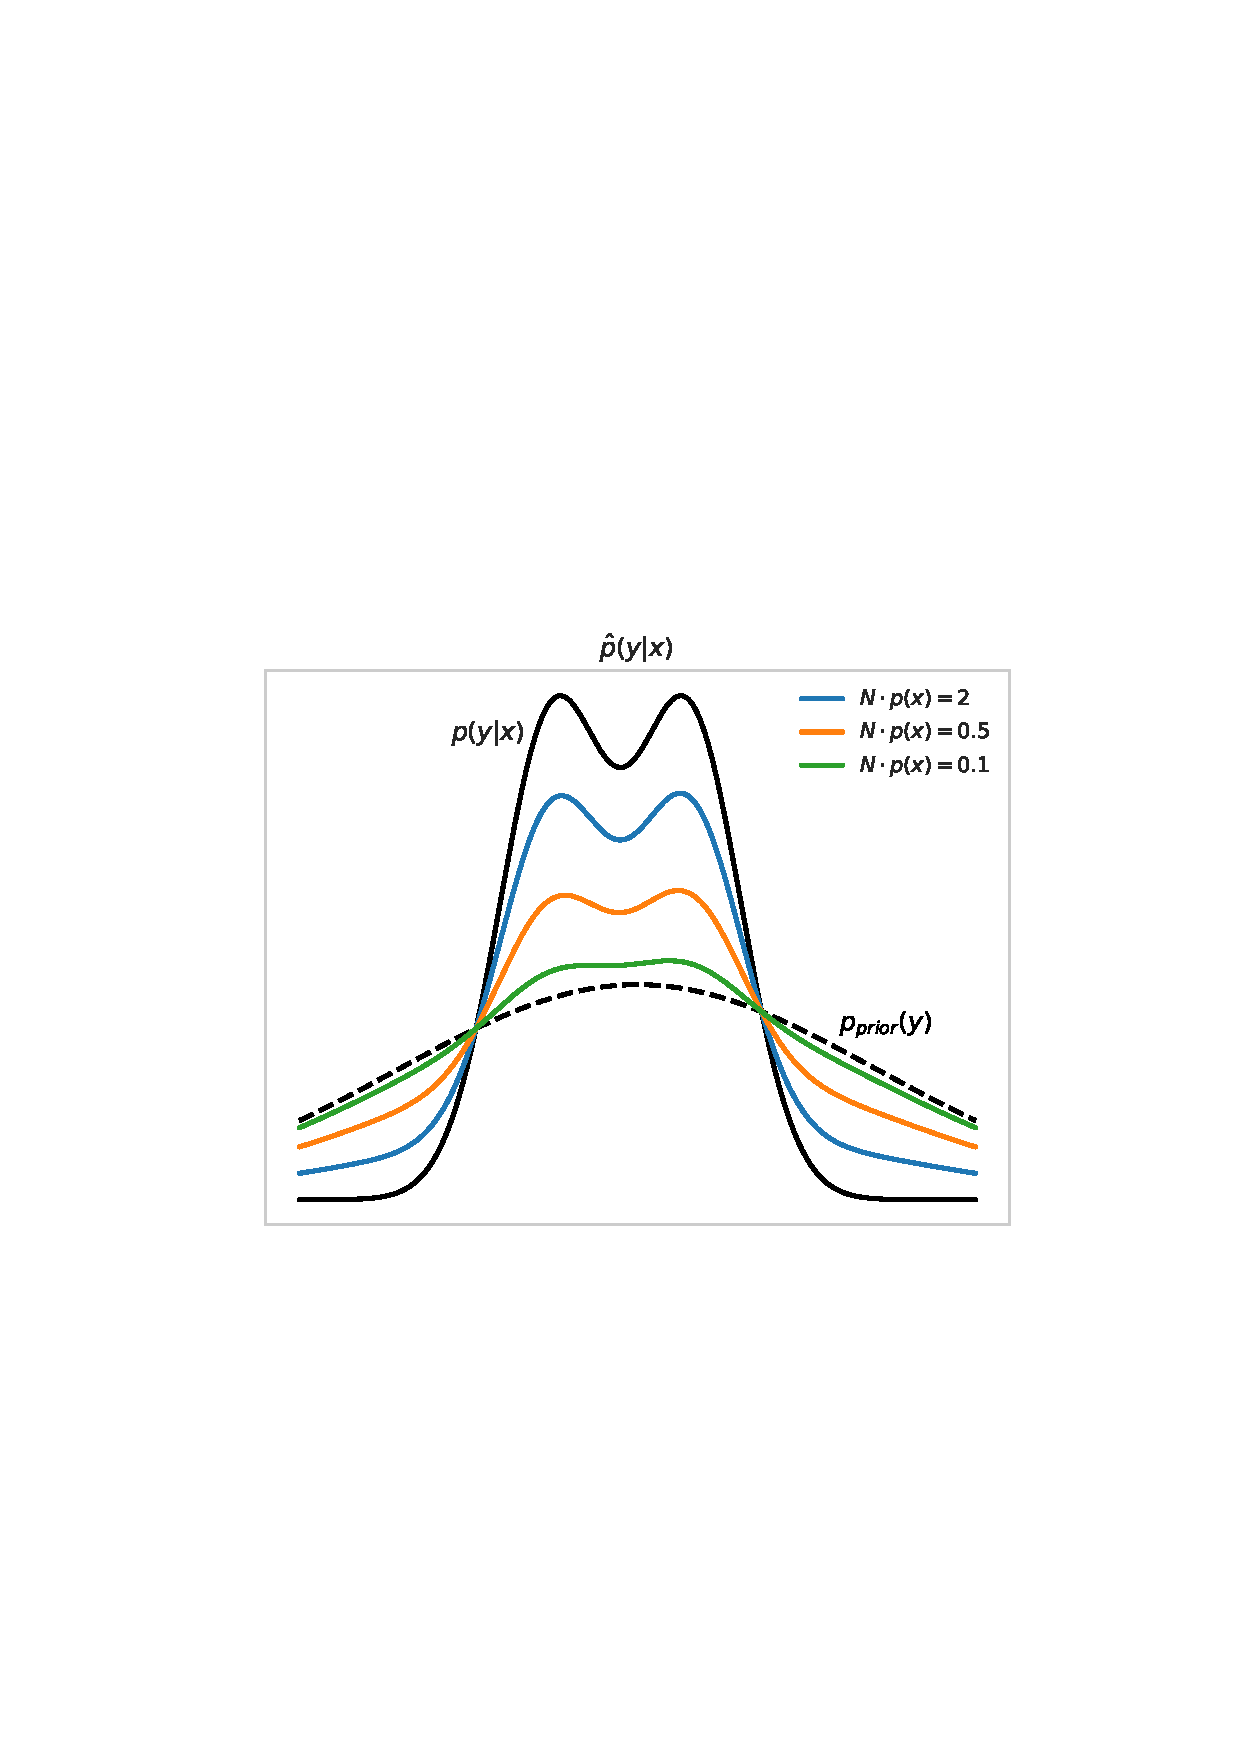
\includegraphics[width=0.45\textwidth]{Pictures/mixture_predictive_bayesian.pdf}
    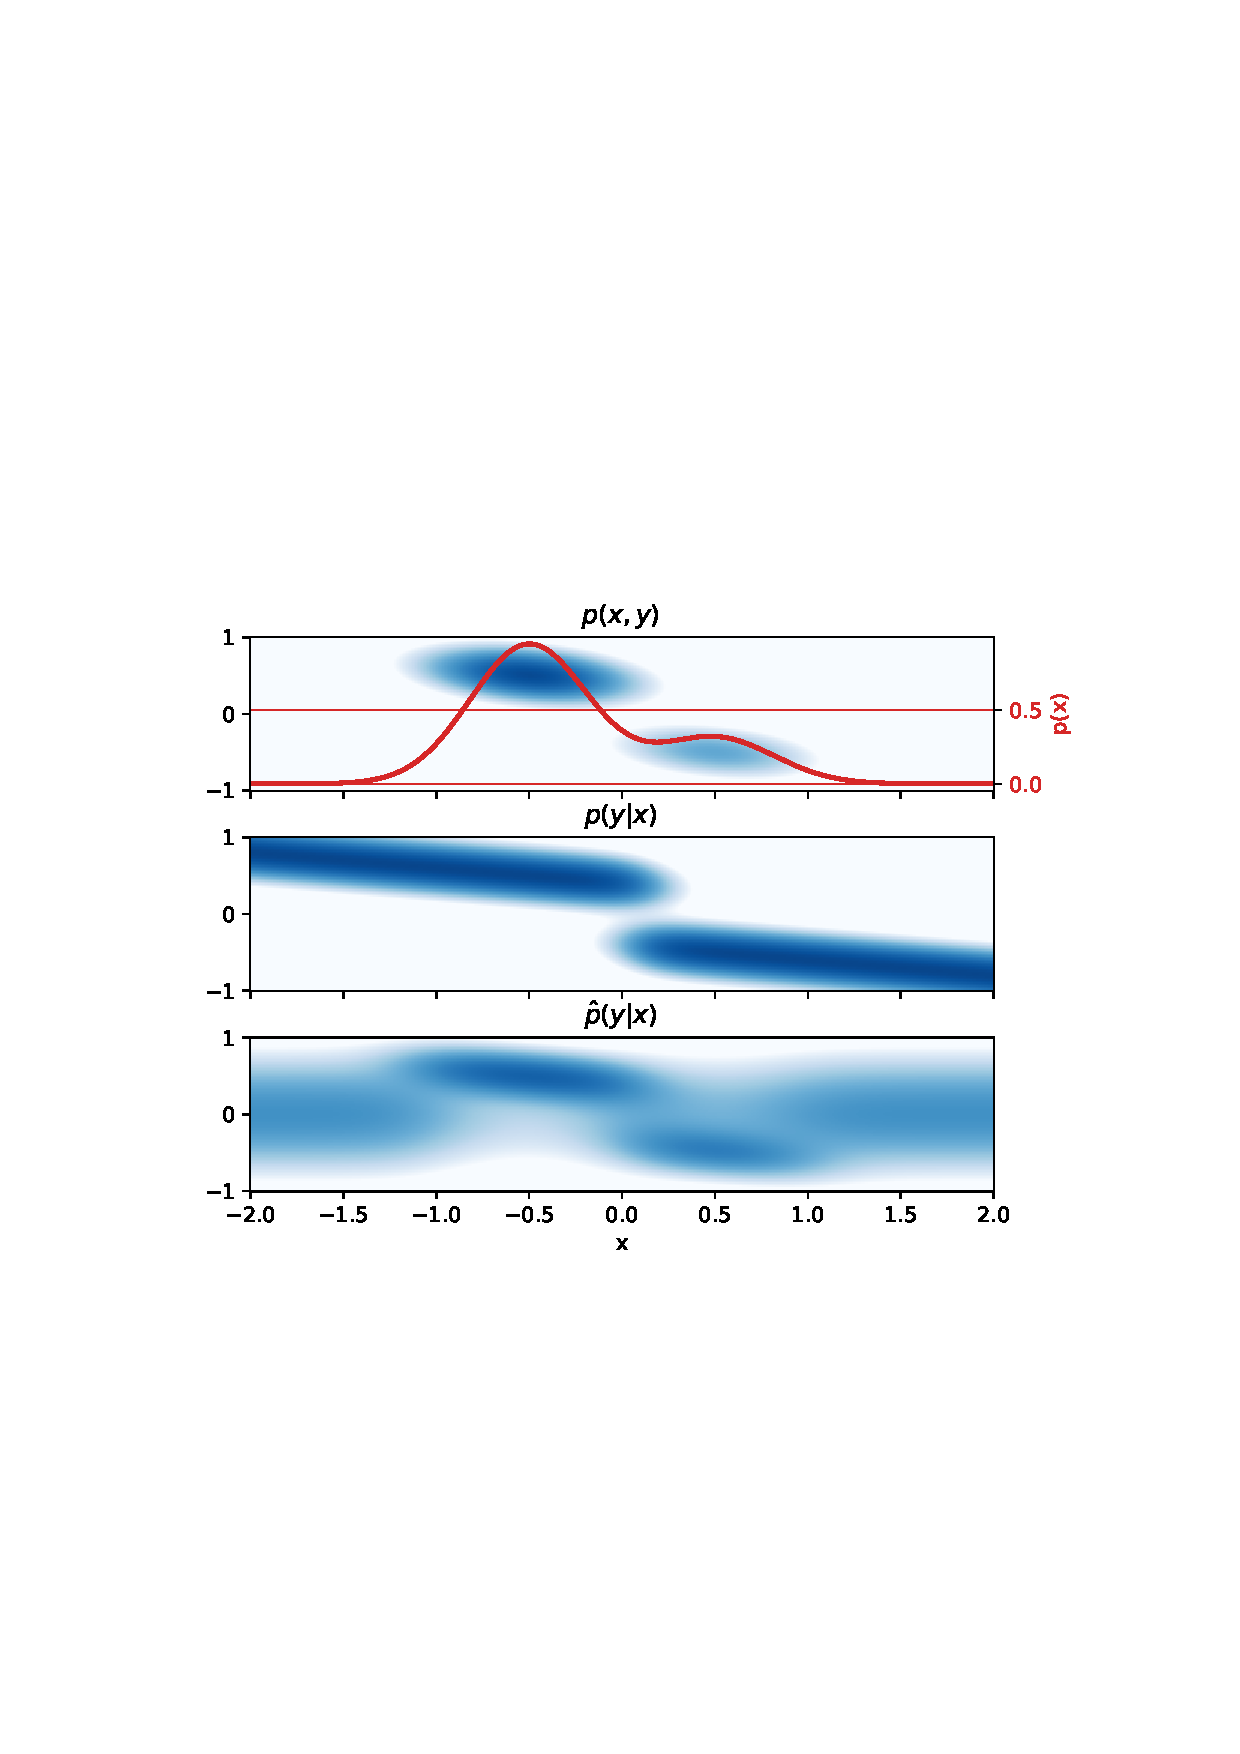
\includegraphics[width=0.45\textwidth]{Pictures/mixture_predictive_bayesian2D.pdf}
    \caption{Left: Illustration of how the preditive distribution is manipulated according
    the the scaling function $S(x) := p(x)\cdot N$. Right: Illustration of why it makes
    sense to manipulate the predictive distribution $p(y|x)$, if there is a small amount of input data
    at a region, then the predictive distribution should collapse into the uncertain prior}
    \label{pred_dist_manipulation}
\end{figure}

\subsubsection{Manipulated predictive mean}
What is the mean prediction of the manipulated predictive distribution?
\begin{align*}
    E_{p_{bayes}(y|x)}[y] &= \int y \cdot \frac{f(n,p(x)) \cdot p(y|x) + \lambda p_{prior}(y)}{Z} dy\\
    &= \left(p(x)\cdot N \cdot E_{p(y|x)}[y] + \lambda \cdot E_{p_{prior}(y)}[y] \right) \frac{1}{Z}\\
    &= \frac{p(x)\cdot N\cdot E_{p(y|x)}[y]}{p(x)\cdot N+\lambda}
\end{align*}

\subsubsection{Manipulated predictive variance}
What is the variance of the manipulated predictive distribution
We first calculate the second moment, 
\begin{align*}
    E_{p_{bayes}(y|x)}[y^2] &= \int y^2 \cdot \frac{p(x)\cdot N \cdot p(y|x) + \lambda p_{prior}(y)}{Z} dy\\
    &= (p(x)\cdot N\cdot E_{p(y|x)}[y^2] + \lambda E_{p_{prior}(y)}[y^2] ) \frac{1}{Z}\\
    &= \frac{p(x)\cdot N \cdot(Var_{p(y|x)}[y]+E_{p(y|x)}[y]^2) + \lambda Var_{p_{prior}(y)}[y]}{p(x)\cdot N+\lambda}
\end{align*}

So the variance is calculated as, 
$$V_{p_{bayes}(y|x)}[y] = E_{p_{bayes}(y|x)}[y^2] - E_{p(x,y)}[y]^2$$

\subsubsection*{implementation}
It is not necessary to calculate the conditional distribution, since, using Bayes rule
$$p(y|x) = \frac{p(x,y)}{p(x)}$$
so gives
$$p_{bayes}(y|x) = \frac{p(x)\cdot N \cdot p(y|x) + \lambda p_{prior}(y)}{Z} = \frac{N \cdot p(x,y) + \lambda p_{prior}(y)}{Z}$$

$$E_{p(x,y)}[y] = \int_y \int_x yp(x,y) dx dy = \int_y y p(y) dy = E_{p(y)}[y]$$